% ===================================================================
%  Week 6 — Session 1: The Frequency Domain (foundations)
% ===================================================================
\documentclass[10pt,aspectratio=169]{beamer}
% ===================================================================
%  Shared Beamer preamble for "Practical Image Processing"
%  English slides. Compile with pdfLaTeX.
% ===================================================================

\usetheme{metropolis}
\usepackage[T1]{fontenc}
\usepackage[utf8]{inputenc}
\usepackage{lmodern}
\usepackage{listings}
\usepackage{tcolorbox}
\usepackage{fontawesome5}
\usepackage{booktabs}
\usepackage{amsmath,amssymb}
\usepackage{tikz}
\usepackage{pgfplots}
\pgfplotsset{compat=1.17}
\usetikzlibrary{arrows.meta,positioning,shapes.geometric,fit,backgrounds,matrix}
\tcbuselibrary{skins,breakable}

% ---- Palette --------------------------------------------------------
\definecolor{coursePrimary}{HTML}{1B4965}   % deep blue
\definecolor{courseAccent}{HTML}{E76F51}    % coral
\definecolor{courseGood}{HTML}{2A9D8F}      % teal
\definecolor{courseBad}{HTML}{C0392B}       % red
\definecolor{courseInfo}{HTML}{2980B9}      % blue
\definecolor{codeBg}{HTML}{F5F6FA}
\definecolor{codeKw}{HTML}{8E44AD}
\definecolor{codeStr}{HTML}{2A9D8F}
\definecolor{codeCom}{HTML}{7F8C8D}

\setbeamercolor{frametitle}{bg=coursePrimary}
\setbeamercolor{progress bar}{fg=courseAccent}
\setbeamercolor{alerted text}{fg=courseAccent}
\metroset{block=fill,sectionpage=progressbar,numbering=fraction}

% ---- Code listings (Python is built into listings) -----------------
\lstdefinestyle{course}{
  backgroundcolor=\color{codeBg},
  basicstyle=\ttfamily\scriptsize,
  keywordstyle=\color{codeKw}\bfseries,
  stringstyle=\color{codeStr},
  commentstyle=\color{codeCom}\itshape,
  numberstyle=\tiny\color{codeCom},
  numbers=left, numbersep=6pt,
  showstringspaces=false, breaklines=true, breakatwhitespace=true,
  tabsize=4, columns=fullflexible,
  frame=single, framesep=4pt, rulecolor=\color{gray!30},
  keepspaces=true, upquote=true, language=Python,
}
\lstset{style=course}
\lstdefinelanguage{bash}{
  keywords={cd,pip,python,venv,source,import}, sensitive=true,
  morecomment=[l]{\#}, morestring=[b]', morestring=[b]",
}

% ---- Reusable callout boxes ----------------------------------------
\newtcolorbox{goodbox}[1][Good practice]{colback=courseGood!8,colframe=courseGood,
  fonttitle=\bfseries,title={\faCheck~#1},boxrule=0.6pt,left=4pt,right=4pt,top=3pt,bottom=3pt}
\newtcolorbox{badbox}[1][Pitfall]{colback=courseBad!8,colframe=courseBad,
  fonttitle=\bfseries,title={\faTimes~#1},boxrule=0.6pt,left=4pt,right=4pt,top=3pt,bottom=3pt}
\newtcolorbox{infobox}[1][Note]{colback=courseInfo!8,colframe=courseInfo,
  fonttitle=\bfseries,title={\faInfoCircle~#1},boxrule=0.6pt,left=4pt,right=4pt,top=3pt,bottom=3pt}
\newtcolorbox{mathbox}[1][Math]{colback=coursePrimary!6,colframe=coursePrimary,
  fonttitle=\bfseries,title={\faCalculator~#1},boxrule=0.6pt,left=4pt,right=4pt,top=3pt,bottom=3pt}

\newcommand{\keyidea}[1]{\begin{alertblock}{Key idea}#1\end{alertblock}}
\newcommand{\term}[1]{\textbf{\color{coursePrimary}#1}}
\newcommand{\code}[1]{\lstinline[basicstyle=\ttfamily\small]|#1|}

% ---- A helper to draw a small pixel grid, cells shaded by value ----
% \pixelgrid{ {10,20,120,200,240}, {30,60,130,180,230}, ... }
\newcommand{\pixelgrid}[1]{%
  \begin{tikzpicture}[font=\scriptsize,scale=0.6]
    \foreach \row [count=\ry] in {#1} {
      \foreach \val [count=\cx] in \row {
        \draw[gray,fill=coursePrimary!8] (\cx,-\ry) rectangle ++(1,-1);
        \node at (\cx+0.5,-\ry-0.5) {\val};
      }
    }
  \end{tikzpicture}}


\title{The Frequency Domain}
\subtitle{Week 6 — Session 1: Seeing images as sums of waves}
\author{Practical Image Processing}
\date{Lecture 6.1 \textbullet\ 60--70 min}

\begin{document}

\maketitle

\begin{frame}{Recap \& today}
  \begin{columns}[T]
    \begin{column}{0.58\textwidth}
      \begin{itemize}
        \item Wk3--5: filters in the \term{spatial} domain (pixels \& kernels).
        \item \alert{Today (Session 1):} a whole new coordinate system for images — the
              \term{frequency} domain. Every image is a sum of waves.
        \item We build the intuition, learn to \emph{read} a spectrum, and do low/high-pass
              filtering by masking.
      \end{itemize}
    \end{column}
    \begin{column}{0.42\textwidth}
      \begin{alertblock}{Why it matters}
        A striped/patterned scan of a meter is nearly impossible to clean spatially — but it's
        a few dots in the frequency domain. (We tackle that in Session 2.)
      \end{alertblock}
    \end{column}
  \end{columns}
\end{frame}

\begin{frame}{Roadmap}\tableofcontents\end{frame}

% ==================================================================
\section{The Fourier idea}
% ==================================================================

\begin{frame}{Any signal = a sum of sine waves}
  \begin{itemize}
    \item \term{Fourier}: any image can be written as a sum of 2D sinusoids of different
          \term{frequency}, \term{orientation}, and \term{amplitude}.
    \item Low frequencies = smooth, slow variation (overall brightness, big shapes).
    \item High frequencies = fast variation (edges, fine texture, noise).
  \end{itemize}
  \begin{mathbox}
    2D DFT: $F(u,v)=\displaystyle\sum_{x=0}^{W-1}\sum_{y=0}^{H-1} f(x,y)\,e^{-j2\pi(ux/W + vy/H)}$
  \end{mathbox}
  \keyidea{The transform doesn't change the image — it re-describes it. Same information,
  different axes: instead of ``brightness at each pixel'' we store ``how much of each wave.''}
\end{frame}

\begin{frame}{1D intuition: building a square wave from sines}
  \begin{columns}[T]
    \begin{column}{0.6\textwidth}
      \begin{center}
      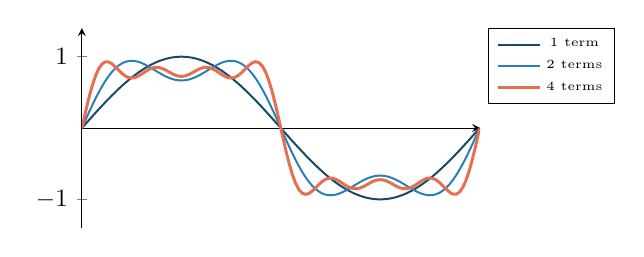
\begin{tikzpicture}[scale=0.9]
        \begin{axis}[width=7.2cm,height=4.4cm,xmin=0,xmax=6.29,ymin=-1.4,ymax=1.4,
            axis lines=middle,xtick=\empty,ytick={-1,1},
            legend style={font=\tiny,at={(1.02,1)},anchor=north west},
            samples=120,domain=0:6.28]
          \addplot[coursePrimary,thick]{sin(deg(x))};
          \addplot[courseInfo,thick]{sin(deg(x)) + sin(deg(3*x))/3};
          \addplot[courseAccent,very thick]
            {sin(deg(x)) + sin(deg(3*x))/3 + sin(deg(5*x))/5 + sin(deg(7*x))/7};
          \legend{1 term,2 terms,4 terms}
        \end{axis}
      \end{tikzpicture}
      \end{center}
    \end{column}
    \begin{column}{0.4\textwidth}
      \begin{itemize}
        \item Add odd harmonics $\sin x + \tfrac13\sin 3x + \tfrac15\sin 5x+\dots$
        \item More terms $\rightarrow$ sharper corners.
        \item \term{Edges need high frequencies}; that is why blurring (dropping high freq)
              rounds corners.
      \end{itemize}
    \end{column}
  \end{columns}
\end{frame}

\begin{frame}{2D sinusoids: frequency, orientation, amplitude}
  \begin{columns}[T]
    \begin{column}{0.33\textwidth}\begin{center}
      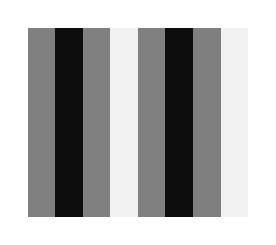
\begin{tikzpicture}
        \foreach \x in {0,...,7}{
          \pgfmathsetmacro{\g}{50+45*sin(deg(3.14159*\x/2))}
          \fill[black!\g] (\x*0.35,0) rectangle ++(0.35,2.4);}
      \end{tikzpicture}\\{\scriptsize horizontal, low freq}
    \end{center}\end{column}
    \begin{column}{0.33\textwidth}\begin{center}
      
\begin{tikzpicture}
        \foreach \x in {0,...,13}{
          \pgfmathsetmacro{\g}{50+45*sin(deg(3.14159*\x))}
          \fill[black!\g] (\x*0.2,0) rectangle ++(0.2,2.4);}
      \end{tikzpicture}\\{\scriptsize horizontal, high freq}
    \end{center}\end{column}
    \begin{column}{0.33\textwidth}\begin{center}
      
\begin{tikzpicture}
        \foreach \y in {0,...,7}{
          \pgfmathsetmacro{\g}{50+45*sin(deg(3.14159*\y/2))}
          \fill[black!\g] (0,\y*0.3) rectangle ++(2.4,0.3);}
      \end{tikzpicture}\\{\scriptsize vertical orientation}
    \end{center}\end{column}
  \end{columns}
  \vspace{4pt}
  A single 2D sinusoid is a set of parallel stripes. Three numbers describe it:
  \term{frequency} (stripe spacing), \term{orientation} (stripe direction), \term{amplitude}
  (contrast). The whole image is a weighted sum of these.
\end{frame}

\begin{frame}{Worked example: a tiny 1D DFT by hand}
  \begin{mathbox}
    Signal $f = [\,4,\;0,\;4,\;0\,]$ (a 2-sample-period stripe). $N=4$.
    $\quad F(u)=\sum_{x=0}^{3} f(x)\,e^{-j2\pi ux/4}$
  \end{mathbox}
  \begin{itemize}
    \item $F(0)=4+0+4+0 = 8$ \hfill (the \term{DC} term = sum = $4\times$ the average).
    \item $F(1)=4\,e^{0}+0+4\,e^{-j\pi}+0 = 4-4 = 0$.
    \item $F(2)=4\,e^{0}+0+4\,e^{-j2\pi}+0 = 4+4 = 8$ \hfill (energy at the \term{highest} freq).
    \item $F(3)=0$ (mirror of $F(1)$).
  \end{itemize}
  \keyidea{$[4,0,4,0]$ alternates every sample $\rightarrow$ all its non-DC energy sits at the
  maximum frequency $u=2$. The numbers match the picture: a fast stripe.}
\end{frame}

% ==================================================================
\section{Reading the spectrum}
% ==================================================================

\begin{frame}{The spectrum of a real plate}
  \begin{columns}[T]
    \begin{column}{0.5\textwidth}\begin{center}
      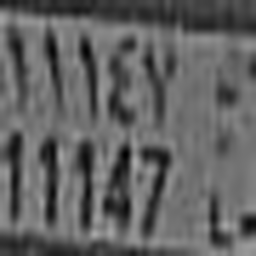
\includegraphics[width=0.8\linewidth]{../assets/gray.png}\\{\scriptsize image (spatial)}
    \end{center}\end{column}
    \begin{column}{0.5\textwidth}\begin{center}
      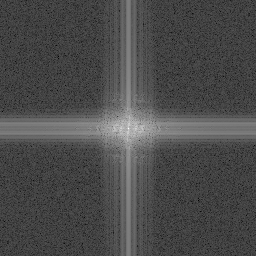
\includegraphics[width=0.8\linewidth]{../assets/spectrum.png}\\{\scriptsize magnitude spectrum (log)}
    \end{center}\end{column}
  \end{columns}
  \vspace{3pt}
  \begin{itemize}
    \item Centre = low frequencies (DC = average brightness). Edges = high frequencies.
    \item Bright lines/points reveal dominant orientations and repeating structure.
  \end{itemize}
\end{frame}

\begin{frame}{Reading the spectrum: three rules}
  \begin{itemize}
    \item The \term{centre} is the average; energy usually concentrates there (natural images are mostly low-freq).
    \item A strong \term{direction} in the image $\rightarrow$ a bright line \emph{perpendicular} to it in the spectrum.
    \item \term{Repeating patterns} (stripes, halftone) $\rightarrow$ isolated bright \term{peaks} off-centre.
  \end{itemize}
  \begin{infobox}
    We take the \code{log} of the magnitude to see anything — the DC term dwarfs everything else.
  \end{infobox}
\end{frame}

\begin{frame}{Why we take the log of the magnitude}
  \begin{columns}[T]
    \begin{column}{0.5\textwidth}
      Raw magnitudes span a huge range. Example values along one row:
      \begin{center}\pixelgrid{{60000,900,300,90,40}}\end{center}
      On a linear scale only the DC pixel is visible; the rest look black.
    \end{column}
    \begin{column}{0.5\textwidth}
      After $20\log_{10}(1+|F|)$:
      \begin{center}\pixelgrid{{95,59,50,39,32}}\end{center}
      \begin{goodbox}
        The $+1$ inside the log avoids $\log 0$. The log compresses 4 orders of magnitude into a
        readable image.
      \end{goodbox}
    \end{column}
  \end{columns}
\end{frame}

\begin{frame}{Centering the DC: \code{fftshift}}
  \begin{columns}[T]
    \begin{column}{0.5\textwidth}\begin{center}
      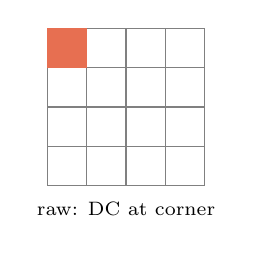
\begin{tikzpicture}[scale=0.5]
        \draw[step=1,gray] (0,0) grid (4,4);
        \fill[courseAccent] (0,3) rectangle (1,4);
        \node at (2,-0.6){\scriptsize raw: DC at corner};
      \end{tikzpicture}
    \end{center}\end{column}
    \begin{column}{0.5\textwidth}\begin{center}
      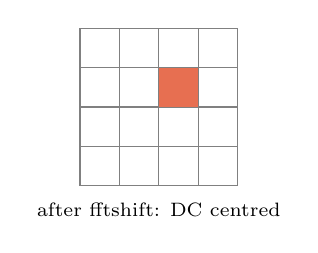
\begin{tikzpicture}[scale=0.5]
        \draw[step=1,gray] (0,0) grid (4,4);
        \fill[courseAccent] (2,2) rectangle (3,3);
        \node at (2,-0.6){\scriptsize after fftshift: DC centred};
      \end{tikzpicture}
    \end{center}\end{column}
  \end{columns}
  \vspace{4pt}
  \begin{itemize}
    \item Raw FFT output puts the zero frequency (DC) at the top-left corner.
    \item \code{fftshift} swaps quadrants so DC lands in the middle — the way we always draw and
          reason about spectra.
    \item Remember to \code{ifftshift} back before the inverse transform.
  \end{itemize}
\end{frame}

\begin{frame}{A gallery of simple spectra}
  \begin{columns}[T]
    \begin{column}{0.33\textwidth}\begin{center}
      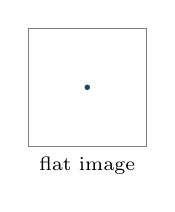
\begin{tikzpicture}[scale=0.5]
        \draw[gray] (0,0) rectangle (3,3);
        \fill[coursePrimary] (1.5,1.5) circle (2pt);
        \node at (1.5,-0.5){\scriptsize flat image};
      \end{tikzpicture}\\{\scriptsize one central dot}
    \end{center}\end{column}
    \begin{column}{0.33\textwidth}\begin{center}
      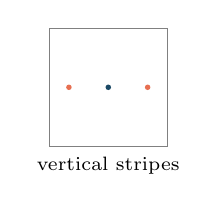
\begin{tikzpicture}[scale=0.5]
        \draw[gray] (0,0) rectangle (3,3);
        \fill[coursePrimary] (1.5,1.5) circle (2pt);
        \fill[courseAccent] (0.5,1.5) circle (2pt);
        \fill[courseAccent] (2.5,1.5) circle (2pt);
        \node at (1.5,-0.5){\scriptsize vertical stripes};
      \end{tikzpicture}\\{\scriptsize DC + symmetric pair}
    \end{center}\end{column}
    \begin{column}{0.33\textwidth}\begin{center}
      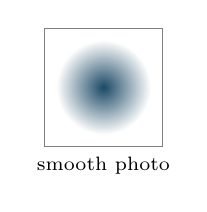
\begin{tikzpicture}[scale=0.5]
        \draw[gray] (0,0) rectangle (3,3);
        \shade[inner color=coursePrimary,outer color=white] (1.5,1.5) circle (1.2);
        \node at (1.5,-0.5){\scriptsize smooth photo};
      \end{tikzpicture}\\{\scriptsize energy hugging centre}
    \end{center}\end{column}
  \end{columns}
  \vspace{4pt}
  Learn these three archetypes and you can read most spectra by inspection.
\end{frame}

\begin{frame}{Symmetry: a real image's spectrum is a mirror}
  \begin{mathbox}
    For a real-valued image, $F(-u,-v) = \overline{F(u,v)}$ (conjugate symmetry).
    So $|F|$ is symmetric through the centre: $|F(-u,-v)| = |F(u,v)|$.
  \end{mathbox}
  \begin{itemize}
    \item Every bright point has an equally bright \term{twin} on the opposite side of the DC.
    \item That is why stripes always show \emph{two} peaks, and why we notch them in pairs (Session 2).
    \item Half the spectrum is redundant — real-FFT routines exploit this to save memory.
  \end{itemize}
\end{frame}

% ==================================================================
\section{Filtering in frequency}
% ==================================================================

\begin{frame}{Low-pass \& high-pass, done in frequency}
  \begin{columns}[T]
    \begin{column}{0.33\textwidth}\begin{center}
      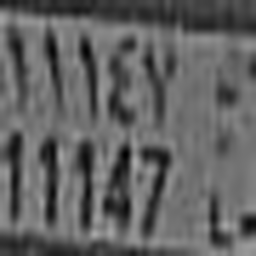
\includegraphics[width=\linewidth]{../assets/gray.png}\\{\scriptsize original}
    \end{center}\end{column}
    \begin{column}{0.33\textwidth}\begin{center}
      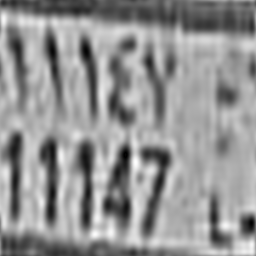
\includegraphics[width=\linewidth]{../assets/lowpass.png}\\{\scriptsize low-pass = blur}
    \end{center}\end{column}
    \begin{column}{0.33\textwidth}\begin{center}
      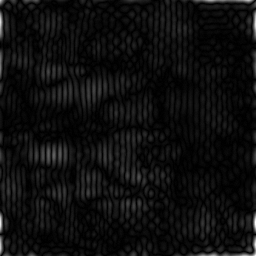
\includegraphics[width=\linewidth]{../assets/highpass.png}\\{\scriptsize high-pass = edges}
    \end{center}\end{column}
  \end{columns}
  \vspace{3pt}
  Keep the centre (low freq) $\rightarrow$ smoothing. Remove the centre (keep high) $\rightarrow$ edges.
  Same effects as Week 3, achieved by \emph{masking} the spectrum.
\end{frame}

\begin{frame}{Convolution theorem: why this matters}
  \begin{mathbox}
    Convolution in space $=$ multiplication in frequency: $f * h \;\longleftrightarrow\; F\cdot H$
  \end{mathbox}
  \begin{itemize}
    \item A big spatial convolution becomes a cheap element-wise multiply in frequency.
    \item For large kernels, FFT-based filtering is much faster ($O(N\log N)$ vs $O(N k^2)$).
    \item It's also \emph{why} the spatial and frequency views are two sides of one coin.
  \end{itemize}
\end{frame}

\begin{frame}{Worked example: when does the FFT pay off?}
  \begin{mathbox}
    Image $N = 1024^2 \approx 10^6$ pixels. Spatial cost $\approx N k^2$; FFT cost $\approx N\log_2 N$.
  \end{mathbox}
  \begin{itemize}
    \item $\log_2 N \approx 20$, so FFT filtering costs $\approx 2\times 10^7$ ops (independent of kernel size).
    \item A $3\times3$ kernel: spatial $\approx 9\times10^6$ ops — \term{spatial wins} for tiny kernels.
    \item A $31\times31$ kernel: spatial $\approx 10^9$ ops — \term{FFT wins} by $\sim 50\times$.
  \end{itemize}
  \keyidea{Break-even is around a $15$--$20$ pixel kernel. Small blur: stay spatial.
  Large blur or a full-image mask: go to frequency.}
\end{frame}

\begin{frame}{Ideal vs smooth filters (ringing)}
  \begin{itemize}
    \item An \term{ideal} sharp cutoff (a hard circle) causes \term{ringing} — ripples near edges.
    \item Smooth cutoffs (\term{Butterworth}, \term{Gaussian}) avoid ringing — the usual choice.
    \item Trade-off: sharper frequency selectivity $\leftrightarrow$ more spatial ringing.
  \end{itemize}
  \begin{badbox}
    A hard frequency mask can add wavy artifacts to a clean image. Prefer a gradual roll-off.
  \end{badbox}
\end{frame}

\begin{frame}{The shape of the roll-off}
  \begin{center}
  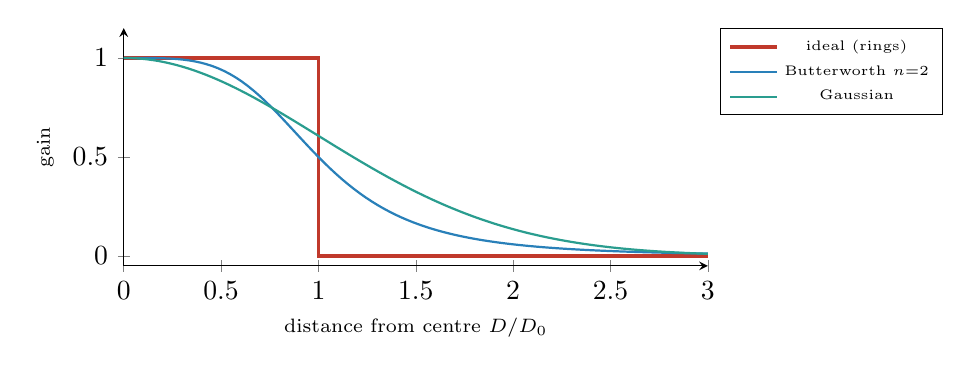
\begin{tikzpicture}
    \begin{axis}[width=9cm,height=4.6cm,xmin=0,xmax=3,ymin=-0.05,ymax=1.15,
        xlabel={\scriptsize distance from centre $D/D_0$},ylabel={\scriptsize gain},
        legend style={font=\tiny,at={(1.02,1)},anchor=north west},
        samples=100,domain=0:3,axis lines=left]
      \addplot[courseBad,very thick,const plot mark left] coordinates {(0,1)(1,1)(1,0)(3,0)};
      \addplot[courseInfo,thick,domain=0.001:3]{1/(1+(x)^(2*2))};
      \addplot[courseGood,thick]{exp(-(x*x)/2)};
      \legend{ideal (rings),Butterworth $n{=}2$,Gaussian}
    \end{axis}
  \end{tikzpicture}
  \end{center}
  The ideal filter's vertical wall is what injects ringing; the smooth curves taper the transition
  and stay artifact-free.
\end{frame}

\begin{frame}[fragile]{Fourier in code}
\begin{lstlisting}[language=Python]
F = np.fft.fftshift(np.fft.fft2(gray))     # to frequency, centre the DC
mag = 20*np.log(np.abs(F) + 1)             # log magnitude for display
# low-pass: keep a central disc
mask = make_circle_mask(gray.shape, r=30)
out = np.abs(np.fft.ifft2(np.fft.ifftshift(F * mask)))  # back to spatial
\end{lstlisting}
  \code{fft2} $\rightarrow$ mask $\rightarrow$ \code{ifft2}. The whole frequency workflow in three steps.
\end{frame}

\begin{frame}{Separability: 2D FFT = rows then columns}
  \begin{mathbox}
    $F(u,v)=\displaystyle\sum_{x}\Big[\underbrace{\sum_{y} f(x,y)\,e^{-j2\pi vy/H}}_{\text{1D FFT of each column}}\Big]e^{-j2\pi ux/W}$
  \end{mathbox}
  \begin{itemize}
    \item The 2D transform \term{separates}: FFT every column, then FFT every row of the result.
    \item This is why the 2D FFT is only $O(N\log N)$ overall, not something worse.
    \item \code{np.fft.fft2} does both passes for you — but knowing it is two 1D sweeps demystifies it.
  \end{itemize}
  \begin{infobox}
    The same separability is why a 2D Gaussian blur can be done as a horizontal then a vertical 1D
    blur (Week 3) — the two domains echo each other.
  \end{infobox}
\end{frame}

\begin{frame}[fragile]{Building the circular mask}
\begin{lstlisting}[language=Python]
def make_circle_mask(shape, r):
    H, W = shape
    cy, cx = H // 2, W // 2                 # centre = DC after fftshift
    Y, X = np.ogrid[:H, :W]
    D = np.sqrt((X - cx)**2 + (Y - cy)**2)  # distance from centre
    return (D <= r).astype(float)           # 1 inside the disc, 0 outside
# high-pass is just the complement:
hp = 1.0 - make_circle_mask(gray.shape, r=30)
\end{lstlisting}
  \begin{infobox}
    Swap \code{D <= r} for a Gaussian \code{np.exp(-(D**2)/(2*r**2))} to get a smooth,
    ring-free roll-off.
  \end{infobox}
\end{frame}

% ==================================================================
\section{In-class exercise}
% ==================================================================

\begin{frame}{\faPen~In-class exercise (10 min)}
  \begin{infobox}[Predict the spectrum]
  \end{infobox}
  For each image, sketch what its magnitude spectrum looks like:
  \begin{enumerate}
    \item A perfectly flat gray image.
    \item Vertical black-and-white stripes.
    \item A photo with lots of fine texture vs a smooth gradient.
    \item Where in the spectrum would you look to detect a repeating scan pattern?
    \item Bonus: for a $31\times31$ blur on a $1024^2$ image, is FFT or spatial faster?
  \end{enumerate}
\end{frame}

\begin{frame}{\faPen~Debrief}
  \begin{itemize}
    \item (1) Flat $\rightarrow$ a single point at the centre (only DC; no variation).
    \item (2) Vertical stripes $\rightarrow$ two symmetric points on the horizontal axis (one frequency).
    \item (3) Fine texture $\rightarrow$ lots of energy far from centre; smooth $\rightarrow$ energy hugging the centre.
    \item (4) Look for isolated bright peaks \emph{off-centre} — that's periodic structure.
    \item (5) FFT: $31^2\approx 960$ ops/pixel spatially vs $\sim 20$ for FFT $\Rightarrow$ FFT wins.
  \end{itemize}
  \keyidea{The spectrum is a map of ``how much of each wave.'' Reading it becomes intuition with practice.}
\end{frame}

% ==================================================================
\section{Wrap-up}
% ==================================================================

\begin{frame}{Pitfalls \& good practice so far}
  \begin{columns}[T]
    \begin{column}{0.5\textwidth}
      \begin{badbox}
        \begin{itemize}
          \item Forgetting \code{fftshift}/\code{ifftshift} $\rightarrow$ a scrambled result.
          \item Displaying $|F|$ without a log $\rightarrow$ an all-black image.
          \item A hard mask $\rightarrow$ ringing.
        \end{itemize}
      \end{badbox}
    \end{column}
    \begin{column}{0.5\textwidth}
      \begin{goodbox}
        \begin{itemize}
          \item Always centre the DC before reasoning.
          \item Use a smooth roll-off (Gaussian/Butterworth).
          \item Take \code{np.abs} of the inverse — round-off leaves a tiny imaginary part.
        \end{itemize}
      \end{goodbox}
    \end{column}
  \end{columns}
\end{frame}

\begin{frame}{What you should now be able to do}
  \begin{itemize}
    \item Explain an image as a sum of waves; hand-compute a tiny DFT.
    \item Read a magnitude spectrum: centre, directions, off-centre peaks.
    \item Low/high-pass filter by masking; choose ideal vs smooth and know why.
    \item Use the convolution theorem to decide spatial vs FFT.
  \end{itemize}
\end{frame}

\begin{frame}{Next session}
  \begin{alertblock}{Session 2 — the killer application}
    \begin{itemize}
      \item \term{Periodic noise}: repeating stripes are two dots in frequency — zap them with a
            \term{notch} filter.
      \item \term{Phase vs amplitude}, the FFT's speed, and the transform family (DCT, wavelets).
      \item \term{Aliasing} and \term{homomorphic} lighting correction, in the frequency view.
      \item Then the week's deliverable.
    \end{itemize}
  \end{alertblock}
\end{frame}

\begin{frame}[standout]
  An image is a sum of waves.\\[4pt]
  \normalsize Change the axes, and hard problems get simple. Next: making that pay off.
\end{frame}

\end{document}
